\section{Numerical study}
\label{sec:numerics}

% Permit related floats to share text pages instead of forcing sparse float pages.
% Keep the 11 pt document text and all table contents unchanged.
\setcounter{topnumber}{3}
\setcounter{bottomnumber}{2}
\setcounter{totalnumber}{4}
\renewcommand{\topfraction}{0.90}
\renewcommand{\bottomfraction}{0.80}
\renewcommand{\textfraction}{0.08}
\renewcommand{\floatpagefraction}{0.75}

We examine the coefficient formulas, their underlying mechanism, and their
implications for averaged models. Controlled additive-noise experiments
isolate the individual coefficients, the extra control contribution, and
its dependence on noise geometry. Shared-objective logistic-regression
experiments examine how client allocation and temporal averaging affect
finite-tail mean displacement. A final post-hoc comparison connects the
observed displacement direction to the analytical curvature--noise vector.

\subsection{Evaluation quantities and experimental settings}
\label{sec:num-protocol}

The controlled experiments use nonlinear strongly convex objectives with
known minimizers and coefficient targets. We estimate the global mean with
the stationary mean-balance identity. Subtracting the shared leading term
and rescaling exposes the second-order coefficient:
\begin{equation}
\label{eq:num-C}
\widehat{\mathcal C}^{\mathcal A}_j
:=\frac{\widehat b^{\mathcal A}_j-(\gamma/N)B_{11,j}}{\gamma^2},
\qquad j=1,2.
\end{equation}
Theorems~\ref{thm:scaf-main} and~\ref{thm:fa-main} predict convergence
to $B_{20}^{\mathcal A}(H)$ as the step size decreases and the client
count increases. The fitted intercept of a linear extrapolation estimates
this limiting coefficient. More details regarding the experimental settings are provided in appendices. Table~\ref{tab:num-controlled-settings}
collects the controlled parameter grids; Tables~\ref{tab:num-run-schedules}
and~\ref{tab:num-inference} give run lengths and interval procedures.
The real-data settings are collected in Table~\ref{tab:num-real-settings}.

\subsection{Controlled tests of analytical predictions}
\label{sec:num-controlled}

We first estimate each algorithm's coefficient and then directly compare
the algorithms. Complementary tests separate client-count dependence,
multidimensional consistency, local-step dependence, and affine-shift
equivalence. The final controlled experiment tests two specific predictions:
cancellation when $T[C]=0$ and invariance of the matched coefficient under
covariance-preserving changes to the noise law.

\subsubsection{Individual stationary-bias coefficients}
\label{sec:num-coefficients}

\paragraph{Design and rationale.}
This experiment checks the explicit $B_{20}^{\Scaf}(H)$ and
$B_{20}^{\FedAvg}(H)$ formulas separately. A two-dimensional objective
with noncommuting Hessian and noise covariance provides a concrete test of
the matrix-valued geometry. Along the joint path $\gamma=1/N$, both
normalized remainder scales decrease together. A smaller-step grid probes
the stability of the $H=4$ estimates.

\paragraph{Results and interpretation.}
Table~\ref{tab:num-attribution-summary} compares the fitted vectors with
the analytical targets. For $H=2$, both algorithms' targets fall within
their simultaneous intervals. For $H=4$, the \FedAvg{} intervals contain
the targets on both grids; the \Scaf{} estimates move closer on the
smaller-step grid, whose intervals also contain both targets. These
comparisons support the predicted coefficient values while showing greater
grid sensitivity for \Scaf{} at $H=4$. Complete interval endpoints are in
Table~\ref{tab:num-core}. The matched-pair rows are interpreted next.

\begin{table}[!htbp]
\centering\small
\setlength{\tabcolsep}{3pt}
\caption{Analytical coefficient vectors and fitted finite-grid intercepts.
Individual rows target $B_{20}^{\mathcal A}(H)$; matched-pair rows target
$B_{20}^{\mathrm{ctrl}}(H)$. P and S denote the primary and smaller-step
joint grids in Table~\ref{tab:num-controlled-settings}. Values are rounded
to seven decimal places; simultaneous intervals are in
Table~\ref{tab:num-core}.}
\label{tab:num-attribution-summary}
\begin{tabular}{@{}lccrr@{}}
\toprule
Study & $H$ & Grid & Target vector & Estimated intercept vector \\
\midrule
\Scaf{} & 2 & P & $(-0.0480040,\,-0.0600050)$ & $(-0.0476713,\,-0.0595811)$ \\
\Scaf{} & 4 & P & $(-0.1520127,\,-0.1900159)$ & $(-0.1502614,\,-0.1874524)$ \\
\Scaf{} & 4 & S & $(-0.1520127,\,-0.1900159)$ & $(-0.1514772,\,-0.1893273)$ \\
\addlinespace
\FedAvg{} & 2 & P & $(-0.0320027,\,-0.0400033)$ & $(-0.0320430,\,-0.0400539)$ \\
\FedAvg{} & 4 & P & $(-0.0960080,\,-0.1200100)$ & $(-0.0959717,\,-0.1198059)$ \\
\FedAvg{} & 4 & S & $(-0.0960080,\,-0.1200100)$ & $(-0.0959727,\,-0.1199590)$ \\
\addlinespace
Paired difference & 2 & P & $(-0.0160013,\,-0.0200017)$ & $(-0.0160363,\,-0.0200366)$ \\
Paired difference & 4 & P & $(-0.0560047,\,-0.0700059)$ & $(-0.0543238,\,-0.0676943)$ \\
Paired difference & 4 & S & $(-0.0560047,\,-0.0700059)$ & $(-0.0559262,\,-0.0698957)$ \\
\bottomrule
\end{tabular}
\end{table}

\subsubsection{Matched contribution of persistent controls}
\label{sec:num-attribution}

\paragraph{Design and rationale.}
To isolate the additional term in Corollary~\ref{cor:attribution},
we compare \Scaf{} and \FedAvg{} using the same initial global model
and indexed noise within each pair. Their shared leading coefficient
cancels in
\begin{equation}
\label{eq:num-D}
\widehat D_j
:=\widehat{\mathcal C}^{\Scaf}_j-\widehat{\mathcal C}^{\FedAvg}_j
=\frac{\widehat b_j^{\Scaf}-\widehat b_j^{\FedAvg}}{\gamma^2}.
\end{equation}
The target is $B_{20}^{\mathrm{ctrl}}(H)$. Common noise reduces sampling
variation in the comparison, making the extra contribution easier to
resolve than by subtracting independently estimated algorithm means.

\paragraph{Results and interpretation.}
Figure~\ref{fig:num-matched-primary} displays the matched estimates and
analytical targets. The $H=2$ intercept intervals contain both targets.
For $H=4$, the smaller-step grid reduces absolute intercept errors by about
$95\%$, although its intervals still exclude the targets. The experiment
therefore resolves a nonzero control-associated contribution and shows
improved coefficient agreement on the finer grid, with a remaining
$H=4$ offset. Appendix~\ref{app:num-h4-diagnostics} examines this offset:
the grid-point residuals scale approximately with $\gamma+1/N$, and their
finite-step, finite-client, and finite-run sources remain unresolved.

\begin{figure}[!htbp]
\centering
\captionsetup[subfigure]{font=small}
\begin{subfigure}[t]{0.49\textwidth}
\centering
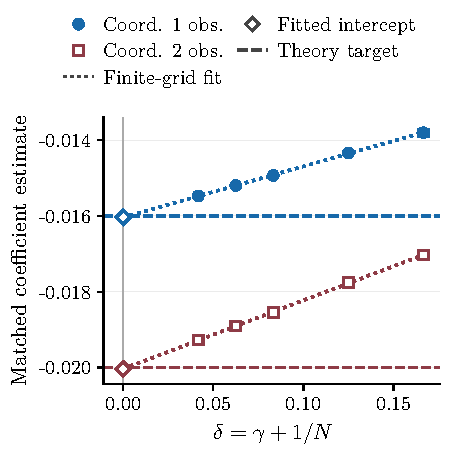
\includegraphics[width=\linewidth]{figures/redrawn/hist_matched_H2.pdf}
\caption{Two local steps}
\end{subfigure}\hfill
\begin{subfigure}[t]{0.49\textwidth}
\centering
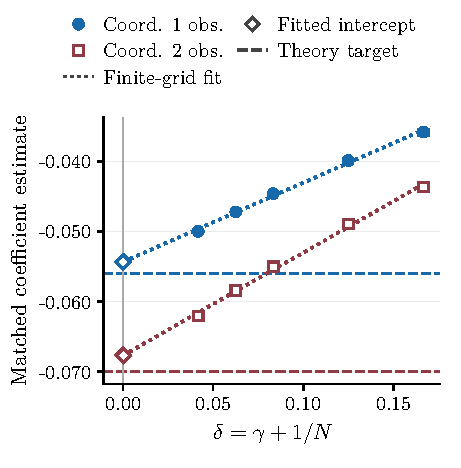
\includegraphics[width=\linewidth]{figures/redrawn/hist_matched_H4.pdf}
\caption{Four local steps}
\end{subfigure}
\caption{Matched \Scaf{}--\FedAvg{} coefficient estimates for (a) $H=2$
and (b) $H=4$ on the primary joint grids. The ordinate is
$\widehat D_j$ from Equation~\eqref{eq:num-D}. Circles and squares show
the two coordinates, dotted lines show finite-grid linear fits, and
dashed horizontal lines give the analytical targets. Open diamonds at
$\delta=0$ mark the fitted intercepts.
Pointwise bars use simultaneous Student-$t$ intervals; intercept bars
use simultaneous seed-block-bootstrap intervals.}
\label{fig:num-matched-primary}
\end{figure}

\subsubsection{Client-count dependence at fixed step size}
\label{sec:num-supporting}

\paragraph{Design and rationale.}
The joint-grid experiment changes $N$ and $\gamma$ together. Here, we hold
the step size and local-step count fixed and increase $N$, isolating the
effect of additional client averaging. A client-independent second-order
term should remain visible as finite-client corrections to the normalized
statistic decrease.

\paragraph{Results and interpretation.}
The normalized \Scaf{} contribution remains visibly nonzero across the
tested client counts (Figure~\ref{fig:E-p2-plateau}). The fitted offsets
from the joint-limit coefficient are reported in
Table~\ref{tab:E-plateau}; the fixed-step expansion permits an
$O(\gamma)$ offset. This result illustrates the distinction between
increasing the client count and reducing the step size: additional clients
suppress the client-dependent term while leaving a residual mean shift.

\begin{figure}[!htbp]
\centering
\captionsetup[subfigure]{font=small}
\begin{subfigure}[t]{0.49\textwidth}
\centering
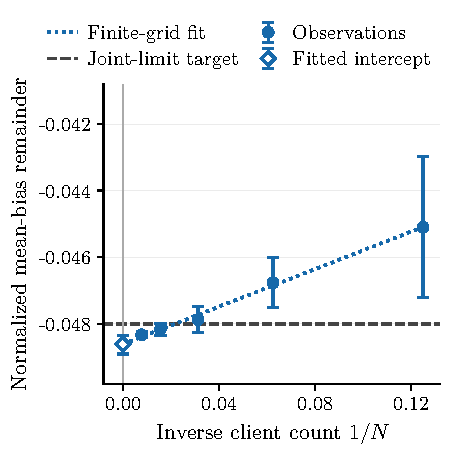
\includegraphics[width=\linewidth]{figures/redrawn/hist_fixed_gamma_coord1.pdf}
\caption{Coordinate 1}
\end{subfigure}\hfill
\begin{subfigure}[t]{0.49\textwidth}
\centering
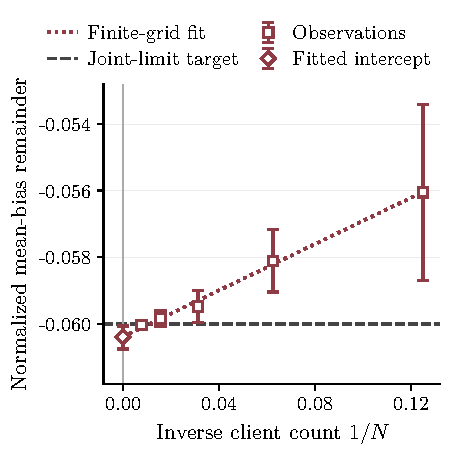
\includegraphics[width=\linewidth]{figures/redrawn/hist_fixed_gamma_coord2.pdf}
\caption{Coordinate 2}
\end{subfigure}
\caption{Client-count dependence at fixed step size, shown by coordinate.
The ordinate is $\widehat{\mathcal C}^{\Scaf}_j$ from
Equation~\eqref{eq:num-C}: the mean-bias estimate after subtracting the
shared $\gamma/N$ term and dividing by $\gamma^2$. Dotted lines give
finite-grid fits and open diamonds their intercepts at $1/N=0$.
Dashed horizontal lines give the joint-limit references
$B_{20}^{\Scaf}(2)$; a fixed step size permits an $O(\gamma)$ offset.
Bars show simultaneous Student-$t$ intervals at grid points and
seed-block-bootstrap intervals for fitted intercepts.}
\label{fig:E-p2-plateau}
\end{figure}

\subsubsection{Multidimensional and coordinate consistency}
\label{sec:num-multidimensional}

\paragraph{Design and rationale.}
A five-dimensional \Scaf{} instance tests the coefficient formula beyond
the primary two-dimensional example, again using noncommuting Hessian and
covariance matrices. A separate rotation check transforms the objective,
noise, and initial state together. The resulting trajectories and
coefficients should transform by the same orthogonal map.

\paragraph{Results and interpretation.}
All ten coordinate targets across $H=2$ and $H=4$ lie within the reported
simultaneous intervals (Table~\ref{tab:E-d5}). The rotation check has
pathwise residuals below $1.6\times10^{-14}$
(Appendix~\ref{app:equivariance-check}). The five-dimensional results
support the coefficient formula across coordinates; the rotation check
confirms that the implementation respects its coordinate transformation.

\subsubsection{Local-step dependence on an independent grid}
\label{sec:num-supp-theory}

\paragraph{Design and rationale.}
The theory assigns different roles to local training length: $B_{11}$ is
shared across $H$, whereas $B_{20}^{\mathrm{ctrl}}(H)$ changes explicitly
with $H$. An independent implementation tests both predictions. Individual
fits of $(N/\gamma)\widehat b$ estimate $B_{11}$ freely. Matched fits on
a Cartesian grid vary $\gamma$ and $1/N$ independently, allowing a direct
comparison with the predicted relation
$B_{20}^{\mathrm{ctrl}}(4)=3.5B_{20}^{\mathrm{ctrl}}(2)$.

\paragraph{Results and interpretation.}
The leading-coefficient intervals contain their targets for $H=1,2,4$;
both algorithms have offsets at $H=8$. The adjusted \Scaf{} $H=8$
versus $H=2$ leading-intercept contrasts exclude zero
(Table~\ref{tab:supp-leading}). For the matched coefficient,
Table~\ref{tab:supp-control} shows target inclusion at $H=2,4$ and target
exclusion at $H=8$. The adjusted $H=4$ minus $3.5(H=2)$ contrast contains
zero in both coordinates. These independent estimates support the predicted
local-step relation at $H=2,4$ and identify $H=8$ as more sensitive to the
fitted grid. Restricted-grid estimates and the separate joint-grid
$H=4$ discrepancy are documented in
Appendix~\ref{app:num-coefficient-results}.

\begin{table}[t]
\centering\small
\caption{Control-coefficient estimates on the independent Cartesian grid.
Each row compares the fitted intercept with $B_{20}^{\mathrm{ctrl}}(H)$.
Intervals are nominal 95\% run-seed intervals.}
\label{tab:supp-control}
\begin{tabular}{@{}ccrrl@{}}\toprule
$H$ & $j$ & Estimate & Target & Nominal interval \\ \midrule
2 & 1 & $-0.01599546$ & $-0.01600134$ & $[-0.01601159,\,-0.01597933]$ \\
2 & 2 & $-0.01999408$ & $-0.02000167$ & $[-0.02001422,\,-0.01997394]$ \\
4 & 1 & $-0.05595226$ & $-0.05600469$ & $[-0.05601109,\,-0.05589342]$ \\
4 & 2 & $-0.06993656$ & $-0.07000586$ & $[-0.07000999,\,-0.06986314]$ \\
8 & 1 & $-0.13962104$ & $-0.14001171$ & $[-0.13983973,\,-0.13940235]$ \\
8 & 2 & $-0.17449119$ & $-0.17501464$ & $[-0.17476345,\,-0.17421894]$ \\
\bottomrule
\end{tabular}
\end{table}

\subsubsection{Affine-shift equivalence}
\label{sec:num-affine}

\paragraph{Design and rationale.}
Proposition~\ref{prop:affine-shift} predicts exact equivalence after
client-specific gradient offsets are absorbed into the controls. We test
this identity by pairing affine-shift and homogeneous recursions with
translated initial controls and identical noise, across several shift
sizes, client counts, and local-step counts.

\paragraph{Results and interpretation.}
Across 24 configurations of 2,000 rounds, the maximum control-state
residual is $1.64313\times10^{-14}$. The numerical recursions therefore
reproduce the predicted state translation to floating-point accuracy.
This illustrates how correction of affine gradient offsets can coexist
with the same stochastic stationary-bias mechanism.

\subsubsection{Contraction cancellation and covariance-matched noise}
\label{sec:num-mechanism-controls}

\paragraph{Design and rationale.}
These tests isolate the specific role of $T[C]$. A nonquadratic
trigonometric objective has $T\ne0$, and the covariance family
$C_\rho=\operatorname{diag}(1+\rho,1-\rho)$ preserves total noise
variance. At $\rho=0$, the contraction vanishes while
$B_{11}=(-0.0125,0)^\top$ remains nonzero, isolating cancellation of the
client-independent coefficient. The positive and negative covariance
controls produce opposite-signed targets. At one fixed covariance,
bounded symmetric and asymmetric noise laws change third and fourth
moments while preserving the predicted coefficients. Unconstrained
Cartesian-grid fits estimate the individual and matched quantities;
the model and laws are given in Appendix~\ref{app:targeted-model}.

\paragraph{Results and interpretation.}
Table~\ref{tab:mechanism-controls} separates the matched null from both
nonzero covariance controls and recovers their predicted signs and
magnitudes. The noise-law contrast is small. In both coordinates, the
null and law-contrast intervals fall within the prespecified
coefficient-resolution margin $\pm0.004375$, equal to $20\%$ of the
nonzero matched target magnitude. Thus the matched increment responds
to covariance geometry and agrees across covariance-matched noise laws
at the reported resolution. Individual first-coordinate null and
law contrasts remain imprecise; one small paired second-coordinate
interval excludes zero while lying within the resolution margin.
Appendix~\ref{app:targeted-results} gives these complementary outcomes
and their sensitivity analyses.

\begin{table}[!htbp]
\centering\small
\setlength{\tabcolsep}{4pt}
\caption{Contraction and noise-law checks for the first coordinate of the
matched coefficient at $H=4$. The covariance controls predict positive,
zero, and negative coefficients; the last row compares noise laws with
identical covariance. Intervals are approximate simultaneous 95\% sampling
intervals for the prespecified 36-scalar family.}
\label{tab:mechanism-controls}
\begin{tabular}{@{}clrrl@{}}
\toprule
$\rho$ & Noise law & Target & Estimate & Simultaneous interval \\
\midrule
$-1/4$ & Symmetric & $0.021875$ & $0.02187858$ & $[0.02184128,\ 0.02191589]$ \\
$0$ & Symmetric & $0.000000$ & $-0.00002056$ & $[-0.00006150,\ 0.00002039]$ \\
$+1/4$ & Symmetric & $-0.021875$ & $-0.02185115$ & $[-0.02189536,\ -0.02180693]$ \\
$+1/4$ & Asymmetric & $-0.021875$ & $-0.02188179$ & $[-0.02193153,\ -0.02183205]$ \\
\midrule
\multicolumn{2}{@{}l}{Symmetric minus asymmetric ($\rho=1/4$)} & $0.000000$ & $0.00003064$ & $[-0.00003564,\ 0.00009692]$ \\
\bottomrule
\end{tabular}
\end{table}

\FloatBarrier

\subsection{Real-data implications of a fixed sampling budget}
\label{sec:num-real}

\paragraph{Design and rationale.}
We examine whether equal aggregate noise makes client allocations
interchangeable. All clients optimize the same a9a logistic-regression
objective, and the total minibatch budget $Nm$ is fixed. At the reference
minimizer $x_{\rm ref}$, the server-averaged noise covariance is
$\Sigma_{\rm ref}/(Nm)$, where $\Sigma_{\rm ref}$ is the single-example
gradient-noise covariance. The local covariance is instead
$\Sigma_{\rm ref}/m$, whose substitution into
Equation~\eqref{eq:ctrl-def} suggests a $\gamma^2/m$ dependence.
This motivates comparing allocations that have equal reference aggregate
noise and different local noise levels.

We measure finite-tail displacement along the preselected unit direction
$v\propto-A_{\rm ref}^{-1}T_{\rm ref}[\Sigma_{\rm ref}]$, with
$A_{\rm ref}=\nabla^2f(x_{\rm ref})$ and
$T_{\rm ref}=\nabla^3f(x_{\rm ref})$:
\begin{equation}
\label{eq:real-projection}
\widehat\delta_v^{\mathcal A}=v^\top(\overline x^{\mathcal A}-x_{\rm ref}),
\end{equation}
Here $\overline x^{\mathcal A}$ averages the per-run tail means across
independent runs. The statistic measures the signed mean displacement
along a direction fixed before the training runs.

\paragraph{Results and interpretation.}
Displacement increases as the same sample budget is distributed among
more clients with smaller local batches (Figure~\ref{fig:real-allocation}).
The $N=128$ minus $N=8$ contrasts are $0.003114$ for \Scaf{} and
$0.002072$ for \FedAvg{}, with adjusted intervals
$[0.002749,0.003478]$ and $[0.001713,0.002431]$. Raw variance estimates
remain near $0.00235$--$0.00236$. Equal reference aggregate covariance
therefore coexists with different finite-tail mean displacements:
the local allocation carries information that server-level covariance
alone does not capture.

\begin{figure}[!htbp]
\centering
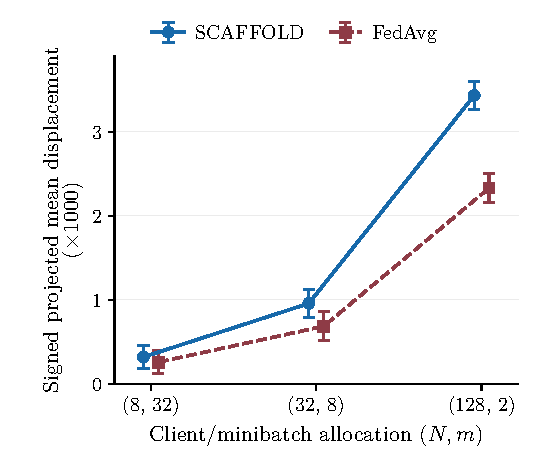
\includegraphics[width=.58\textwidth]{figures/redrawn/real_R0_allocation.pdf}
\caption{Finite-tail mean displacement under a fixed sampling budget.
Each category gives a client-count/minibatch allocation $(N,m)$ with
$Nm=256$. The ordinate is the signed projection in
Equation~\eqref{eq:real-projection}, scaled by $10^3$.
Bars are nominal 95\% run-seed intervals; small offsets distinguish
the algorithms at the same allocation.}
\label{fig:real-allocation}
\end{figure}

The training-configuration comparison in Table~\ref{tab:supp-policy}
provides a complementary interpretation. Reducing $\gamma$ lowers both
displacement and raw variance; reducing $H$ lowers displacement with
much less variance change. These are comparisons under the run schedules
in Table~\ref{tab:num-run-schedules}. The disjoint IID and label-skew
results in Appendix~\ref{app:supp-real} additionally show how
heterogeneity-induced drift correction can dominate the algorithm
difference when the common-objective condition is relaxed.

\begin{table}[t]
\centering\small
\caption{Step-size and local-step comparisons for the shared objective at
$N=32,m=8$. All entries are multiplied by $10^3$.
$\widehat\delta_v$ is signed finite-tail mean displacement and
$\widehat V$ is raw-checkpoint parameter variance.
S: SCAFFOLD; F: FedAvg.}
\label{tab:supp-policy}
\begin{tabular}{@{}lrrrr@{}}\toprule
Setting & $\widehat\delta_v^{\rm S}$ & $\widehat\delta_v^{\rm F}$ & $\widehat V^{\rm S}$ & $\widehat V^{\rm F}$ \\ \midrule
$H=4,\ \gamma=\gamma_b$ & $0.9567$ & $0.6851$ & $2.3621$ & $2.3613$ \\
$H=4,\ \gamma=\gamma_b/2$ & $0.3547$ & $0.2796$ & $1.1723$ & $1.1722$ \\
$H=4,\ \gamma=\gamma_b/4$ & $0.0622$ & $0.0420$ & $0.5860$ & $0.5860$ \\
$H=2,\ \gamma=\gamma_b$ & $0.3402$ & $0.2474$ & $2.3601$ & $2.3599$ \\
\bottomrule
\end{tabular}
\end{table}

\FloatBarrier

\subsection{Model averaging changes the error decomposition}
\label{sec:num-averaging}

\paragraph{Design and rationale.}
Under stationarity, temporal averaging preserves the expected model
while potentially reducing variance. We therefore examine whether
mean displacement becomes a larger share of parameter error when
successive global models are averaged.
We use the same shared-objective runs and average successive global
models within each run over nested windows. Let $Y_{r,K}^{\mathcal A}$
be run $r$'s output averaged over its last $K$ equal-length batches.
Independent runs supply repeated outputs, while the windows share a
common endpoint. Table~\ref{tab:num-real-settings} gives the window
lengths and computational budget.

For a random output $Y_K^{\mathcal A}$ of this finite-window procedure,
\begin{equation}
\label{eq:e4-finite-window-mse}
\mathbb E\|Y_K^{\mathcal A}-x_{\rm ref}\|^2
=\|\mathbb E[Y_K^{\mathcal A}]-x_{\rm ref}\|^2
+\operatorname{tr}\operatorname{Cov}(Y_K^{\mathcal A}).
\end{equation}
We estimate squared mean displacement by the sampling-corrected cross-run
statistic $\widehat U_K$ and averaged-output variance by $\widehat V_K$.
Their sum is the estimated parameter MSE. Sampling correction allows
$\widehat U_K$ to be negative with finitely many runs; the plots retain
these values. Appendix~\ref{app:e4-averaging} gives the estimators.

\paragraph{Results and interpretation.}
In the primary allocation, mean displacement accounts for only about
$0.50\%$ and $0.23\%$ of raw-checkpoint parameter MSE for \Scaf{} and
\FedAvg{}, respectively. Figure~\ref{fig:e4-averaging} shows how this
composition changes after averaging. From $K=1$ to $64$, averaged-output
variance decreases about 57-fold. At $K=64$, the mean-displacement shares
reach $68.1\%$ and $49.5\%$, with simultaneous intervals
$[62.6\%,73.7\%]$ and $[41.1\%,57.9\%]$. Systematic displacement
therefore becomes a substantial part of the averaged-model error in
this experiment, even though individual checkpoints are variance-dominated.

\begin{figure}[!htbp]
\centering
\captionsetup[subfigure]{font=small}
\begin{subfigure}[t]{0.49\textwidth}
\centering
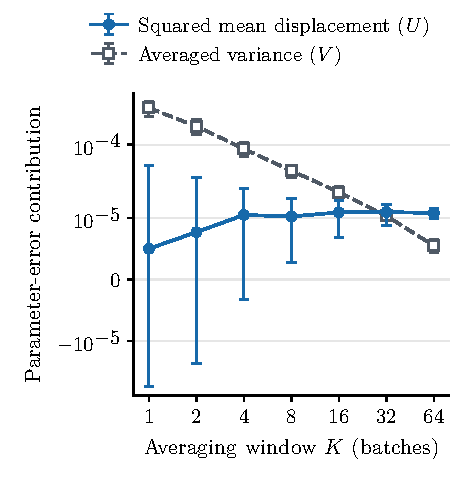
\includegraphics[width=\linewidth]{figures/redrawn/e4_averaging_scaffold.pdf}
\caption{SCAFFOLD}
\end{subfigure}\hfill
\begin{subfigure}[t]{0.49\textwidth}
\centering
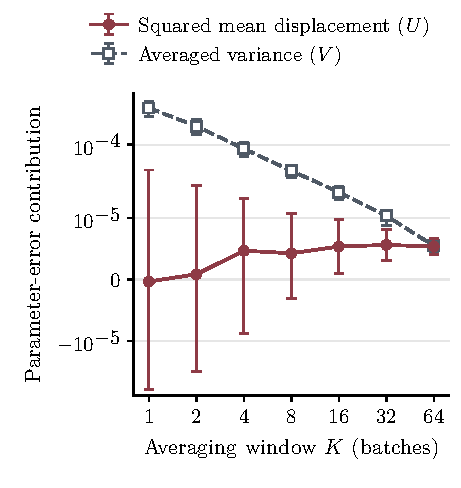
\includegraphics[width=\linewidth]{figures/redrawn/e4_averaging_fedavg.pdf}
\caption{FedAvg}
\end{subfigure}
\caption{Parameter-error decomposition after temporal model averaging.
The panels compare estimated squared mean displacement $\widehat U_K$
with averaged-output variance $\widehat V_K$ over windows of $K$ batches
in the primary shared-objective configuration. Each batch contains 1,280
rounds. Bars are approximate simultaneous 95\% primary-family intervals.
The symmetric-log axis is linear between $-10^{-5}$ and $10^{-5}$ and
retains negative sampling-corrected estimates and intervals crossing zero.}
\label{fig:e4-averaging}
\end{figure}

At the longest window, the \Scaf{}-minus-\FedAvg{} parameter-MSE
contrast is $6.39\times10^{-6}$, with interval
$[5.83,6.95]\times10^{-6}$, mainly associated with squared mean
displacement. The corresponding training-gap contrast is
$3.64\times10^{-7}$, while \Scaf{} has lower held-out log loss by
$3.27\times10^{-5}$. Thus parameter error and predictive loss respond
differently. The averaging result concerns finite-tail outputs;
Appendix~\ref{app:e4-averaging} reports the remaining temporal uncertainty.

\FloatBarrier

\subsection{Directional agreement beyond the additive-noise model}
\label{sec:num-directional}

\paragraph{Design and rationale.}
We examine whether the curvature--noise geometry helps explain the
algorithmic mean displacement under natural minibatch noise. The post-hoc
comparison substitutes the reference-objective quantities from
Section~\ref{sec:num-real} into the analytical expression:
\begin{equation}
\label{eq:e5-proxy}
p_{\gamma,H,m}
=-\frac{\gamma^2}{m}\,\kappa(H)\,A_{\rm ref}^{-1}T_{\rm ref}[\Sigma_{\rm ref}],
\qquad \kappa(H)=\frac{(H-1)(2H-1)}{12H}.
\end{equation}
The observed difference is
$\widehat\Delta_K=R^{-1}\sum_r(Y_{r,K}^{\Scaf}-Y_{r,K}^{\FedAvg})$
over $R=12$ paired runs. The proxy is computed directly from the objective
and reference covariance. Comparing all 124 coordinates tests its
geometric alignment with the observed mean difference. Cosine measures
directional agreement; projection ratio and relative residual measure
amplitude agreement and vector mismatch. Because both algorithms'
second-order terms share the same analytical direction, the amplitude and
local-step comparisons provide information beyond directional alignment.

\paragraph{Results and interpretation.}
At the designated longest window, the six nonzero-proxy configurations
have cosines $0.9965$--$0.9993$, projection ratios $0.716$--$0.938$, and
relative residuals $0.089$--$0.291$ (Table~\ref{tab:e5-bridge}). All six
proxy norms exceed the observed norms. At fixed $H,N,m$, reducing
$\gamma$ moves the projection ratio toward one and decreases the residual.
Alternative fixed directions have lower cosine estimates
(Appendix~\ref{app:e5-bridge}). The analytical geometry thus describes
the observed direction more accurately than its amplitude.

\begin{table}[!htbp]
\centering\small
\setlength{\tabcolsep}{5pt}
\caption{Post-hoc comparison of the analytical proxy $p=p_{\gamma,H,m}$
and the 124-dimensional finite-tail mean difference $\widehat\Delta_K$
at $K=64$. Cosine $=p^\top\widehat\Delta_K/(\|p\|\|\widehat\Delta_K\|)$;
projection ratio $=p^\top\widehat\Delta_K/\|p\|^2$;
relative residual $=\|\widehat\Delta_K-p\|/\|p\|$.
All six nonzero-proxy configurations are shown; the $H=1$ checks and
sampling intervals are in Appendix~\ref{app:e5-bridge}.}
\label{tab:e5-bridge}
\begin{tabular}{@{}rrrrrrr@{}}
\toprule
$H$ & $N$ & $m$ & $\gamma/\gamma_b$ & Cosine & \shortstack{Projection\\ratio} & \shortstack{Relative\\residual} \\
\midrule
2 & 32 & 8 & $1$ & $0.997719$ & $0.938327$ & $0.088505$ \\
4 & 8 & 32 & $1$ & $0.996500$ & $0.715730$ & $0.290542$ \\
4 & 32 & 8 & $1/4$ & $0.997252$ & $0.935781$ & $0.094644$ \\
4 & 32 & 8 & $1/2$ & $0.998972$ & $0.867499$ & $0.138225$ \\
4 & 32 & 8 & $1$ & $0.998994$ & $0.784711$ & $0.218151$ \\
4 & 128 & 2 & $1$ & $0.999254$ & $0.796703$ & $0.205615$ \\
\bottomrule
\end{tabular}
\end{table}

The local-step comparison further separates these two aspects of agreement:
at the base step size and $N=32,m=8$, the observed $H=4/H=2$ projected
ratio is $2.927$, compared with the analytical ratio $3.5$.
Together, the results give a directional explanation of the finite-tail
algorithm difference while identifying quantitative departures in magnitude
and local-step scaling. Appendix~\ref{app:e5-bridge} gives the sampling
intervals and window sensitivity.

